\section{The Gambler's Ruin Problem}
Consider a gambler who starts with an initial fortune and then on each successive gamble
either wins $\$1$ or loses $\$1$ independent of the past with probabilities $p$ and $q = 1-p$ respectively.
The gambler's objective is to reach a total fortune of $\$N$, without first getting ruined (running out of money). If the gambler succeeds,
then the gambler is said to win the game. In any case, the gambler stops playing after winning
or getting ruined, whichever happens first. Let the gambler starts with $\$i$ where $0 < i < N$.

Let $X_{n}$ denote the total fortune after the $n$th gamble. Then $X_{0}=i$, \\
Then the process $ \{X_{n},n=0,1,2,\ldots,N\} $ is a Markov chain With 
transition probabilities
\begin{align*}
    p_{00} &= p_{N N} = 1,\\ 
    p_{i,i+1} &= p = 1-p_{i,i-1} \ \ i=1,2,\ldots,N-1
\end{align*}

This Markov chain has three classes, classes are $ \{0\},\ \{1,2,\ldots,N-1\}\ \&\ \{N\} $ the first and third class being recurrent and 
second transient. Since all each transient state is only visited finitely often, it follows that after some finite amount of time, the gambler
will either wins $ \$N $ or go broke.

Since the game stops when either $X_{n} = 0$ or $X_{n} = N$, let
\[
    \tau_{i} = \min{\{n\ge 0: X_{n}\in\{0,N\}|X_{0}=i\}} 
\]
denote the time at which the game stops when $ X_{0} = i $. If $ X_{\tau_{i}} = N $, then the gambler wins of $ X_{\tau_{i}} = 0 $ gambler is ruin.

Let $ P_{i} = \mathbf{P}(X_{\tau_{i}} = N) $ denotes the probability that the gambler wins when $ X_{0} = i $ clearly $ P_{0} = 0 $ and $ P_{N} = 1 $ 
by definition, (Here $ p_{00}=1  $ and $ p_{N N}=1 $ then state 0 and $ N $ is absorbing state.) 
we next proceed to compute $P_i$, $1 \le  i \le  N - 1$. By conditioning on the outcome of the initial play of the game, we obtain,
\[
    P_{i} = pP_{i+1} + qP_{i-1}, \ \ i=1,2,\ldots,N-1,
\]
Since, $ p + q = 1 $ we get, 
\begin{align*}
    pP_{i} + qP_{i} &= pP_{i+1} + qP_{i-1}\\ 
    P_{i+1} - P_{i} &= \frac{q}{p}(P_{i}-P_{i-1}), \ \ 0<i<N,
\end{align*}
In particular, $ P_{2}-P_{1}=(q/p)(P_{1}-P_{0})=(q/p)P_{1} $ (since, $ P_{0} = 0 $) So that,\\ 
$ P_{3}-P_{2}=(q/p)(P_{2}-P_{1}) = (q/p)^{2}P_{1}$, And hence,
\begin{equation*}
    P_{i+1} -P_{i} = \left( \frac{q}{p} \right)^{i}P_{1}\ \  0<i<N.
\end{equation*}

\begin{align*}
    P_{i+1} -P_{1} &= \sum_{k=1}^{i} (P_{k+1}-P_{k})\\ 
    P_{i+1} -P_{1} &= \sum_{k=1}^{i}\left(\frac{q}{p}\right)^{k}P_{1}  \\
    P_{i+1} &= P_{1} + \sum_{k=1}^{i}\left(\frac{q}{p}\right)^{k}P_{1} =  P_{1}\sum_{k=0}^{i}\left( \frac{q}{p} \right)^k
\end{align*}
Then we get, 
\[
            P_{i+1}  =  \begin{cases}
                P_{1}\frac{1-\left(\frac{q}{p}\right)^{i+1}}{1-\left(\frac{q}{p}\right)} \ \text{ if } p\neq q;\\ 
                P_{1}(i+1) \ \text{ if } p=q=0.5
            \end{cases} \numberthis
\]

Choosing $ i=N-1 $ we get and using  $ P_{N} =1 $ we get,
\[
    1=P_{N}=
    \begin{cases}
        P_{1}\frac{1-\left(\frac{q}{p}\right)^{N}}{1-\left(\frac{q}{p}\right)} \ \text{ if } p\neq q;\\ 
        P_{1}N \ \text{ if } p=q=0.5
    \end{cases}
\]
Hence we get, $ P_{1} = 1/N $ when $ p=q=0.5 $ and  $ P_{1} = \frac{1-(q/p)}{1-(q/p)^{N}} $ Then,
\[
    P_{i}=
    \begin{cases}
        \frac{1-(\frac{q}{p})^{i}}{1-(\frac{q}{p})^{N}}, \ \text{ it } p\neq q;\\ 
        \frac{i}{N} \ \text{ if } p=q=0.5 
    \end{cases} \numberthis \label{probability of ruin or win}
\]

\subsection{Becoming infinitely rich or getting ruined}
If $ p>0.5 $, Then  $ \frac{q}{p}<1 $ from \cref{probability of ruin or win} we get,
\[
    \lim_{N \to \infty} P_{i} = 1-\left(\frac{q}{p}\right)^{i} >0 
\]
i.e. if $ p>0.5 $, there is a positive probability that the gambler will never get ruined but instead will become infinitely rich as $ N\to \infty $.

If $p\le 0.5$ then $ \frac{q}{p}\ge 1 $ thus from \cref{probability of ruin or win}
\[
    \lim_{N \to \infty} P_{i} = 0, \ \ \ p\le 0.5
\]
i.e. if $p \le 0.5$ (each gamble is not in his favor), then with probability one the gambler will get ruined $ N\to \infty $.

\begin{example}[Random walk hitting probabilities]
    Ellen bought a share of stock for $\$10$, and it is believed that the stock price moves (day by day) 
    as a simple random walk with $p = 0.55$. What is the probability that Ellen's
    stock reaches the high value of $\$15$ before the low value of $\$5$? 

    What is the probability that Ellen will become infinitely rich?
\end{example}

\textbf{Solution: } Let us define,
$ P(a) = \mathbf{P}\left(X_{n} \text{ hits }a \text{ before hitting } b\right)$ 

We want to calculate the probability that the stock goes up by 5 before going down by 5.

By letting $ a=5 $ and $ b=5 $ and $ N=a+b=10 $, we can imagine a gambler who started with $ \$5 $ and want to win $ \$5 $
before going broke. So we can compute $P(a)$ by casting the problem into the framework of the gamblers ruin problem: 
$ P(a) = P_{5} $ and $ N=10 $. Then,
\[
    P(5) = P_{5} = \frac{1-\left(\frac{0.45}{0.55}\right)^{5}}{1-\left(\frac{0.45}{0.55}\right)^{10}} = \frac{1-(0.82)^{5}}{1-(0.85)^{10}} = 0.73
\]

To see Ellen will ever be infinity rich we make  $ N\to\infty $ and started gamblers ruin problem at $ \$10 $ then,
\[
    \lim_{N\to\infty}P_{10} = 1 - (q/p)^{10} = 1 - (0.82)^{10} = 0.86
\]


\subsection{Gambler's Ruin Problem Simulation}
We can nicely make a simulation of Gambler's ruin problem And observe the output of it.

\textbf{Observation: }
\begin{itemize}
    \item When $ p=0.45 $ The Gambler will be ruined after 384 games.
    \item When $ p=0.51 $ The Gambler will reach his fortune after 4412 games.
\end{itemize}


\begin{figure}[H]
    \centering
    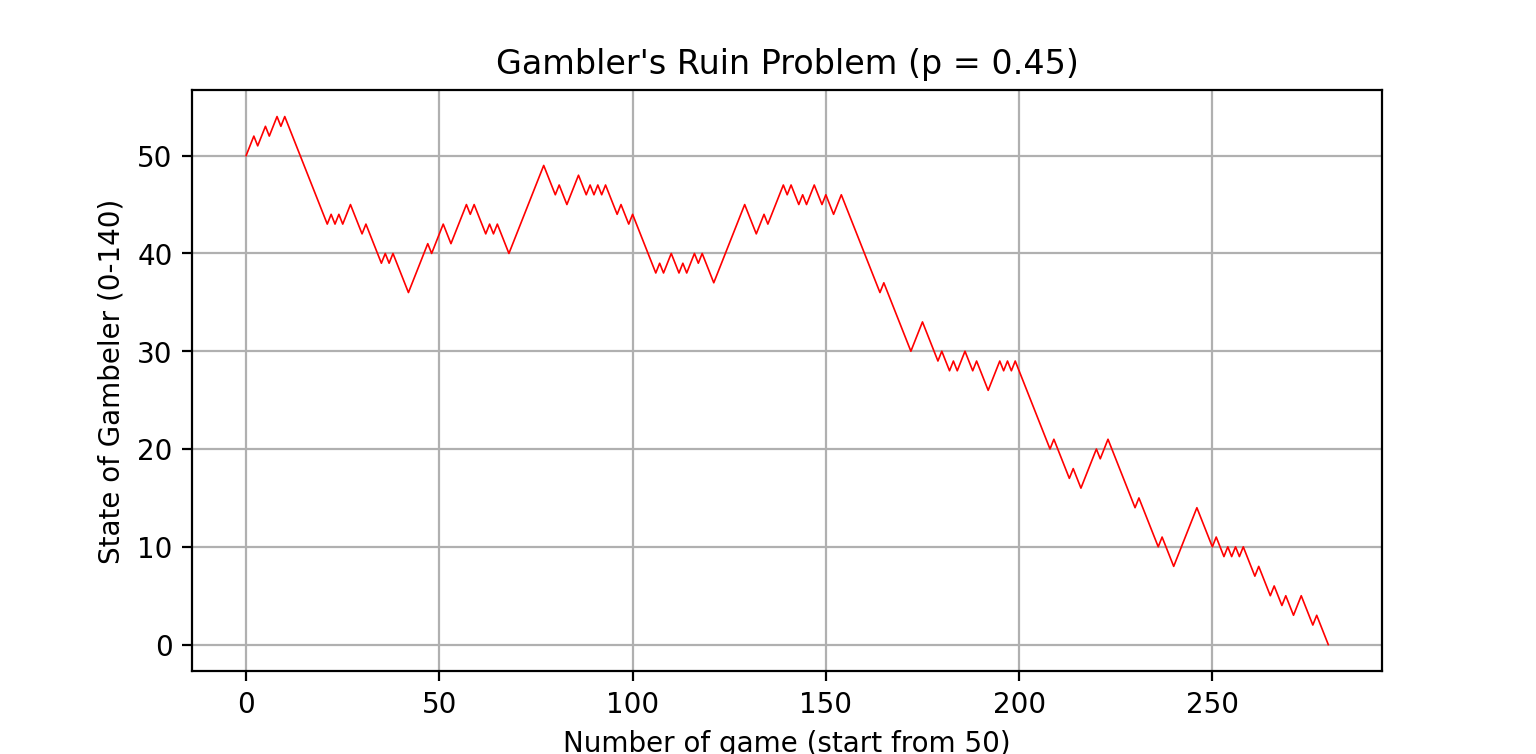
\includegraphics[width=0.8\textwidth]{pic/GR0.45.png}
    \caption{Gambler's Ruin Problem with $( p=0.45 )$}
\end{figure}

\makeatletter
\setlength{\@fptop}{0pt}
\makeatother

\begin{figure}[H]
    \centering
    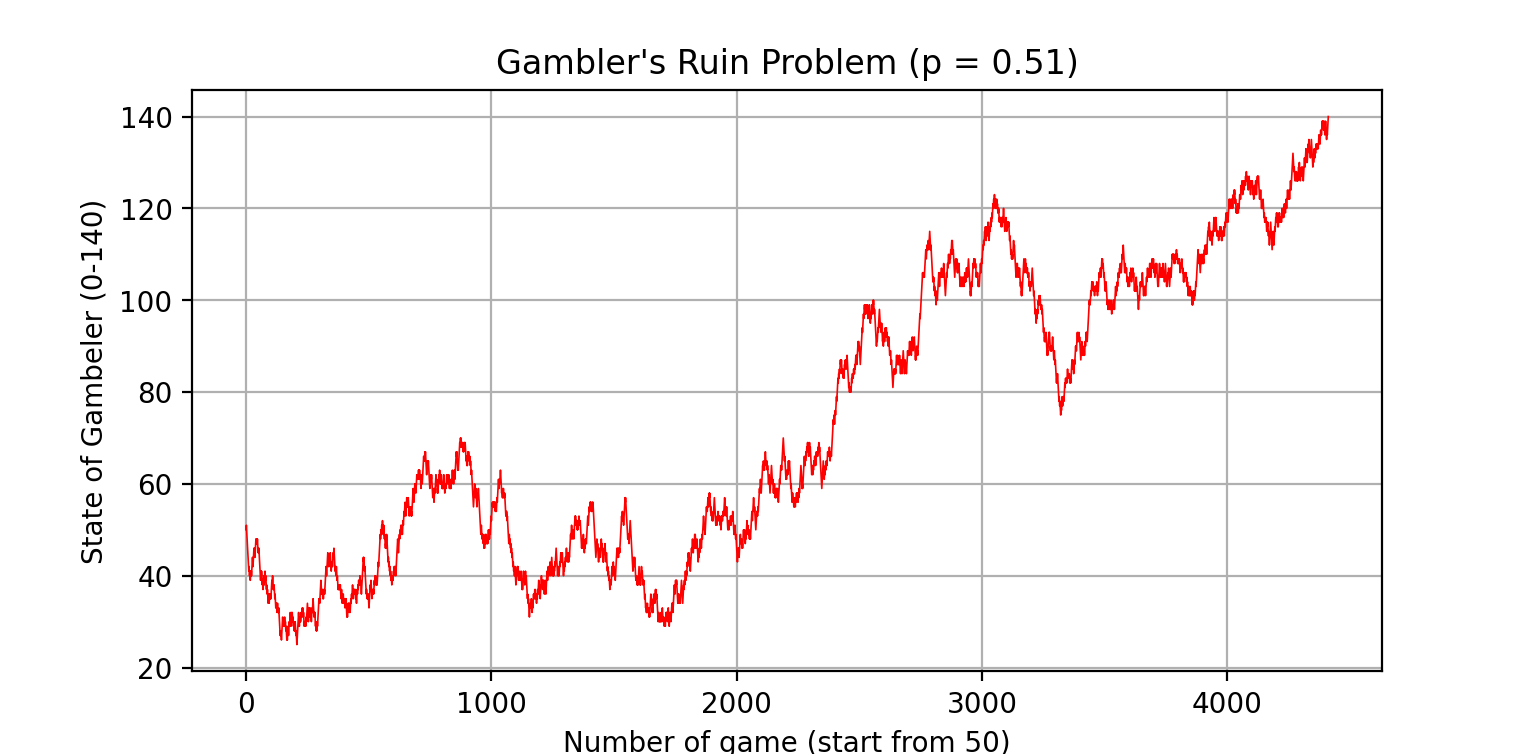
\includegraphics[width=0.8\textwidth]{pic/GR0.51.png}
    \caption{Gambler's Ruin Problem with $( p=0.51 )$}
\end{figure}

